\documentclass[11pt]{article}
\usepackage[utf8]{inputenc}
\usepackage{amssymb, amsmath, amsthm, changepage, graphicx, caption, subcaption}

\graphicspath{{./images/}}

\title{MAT240 Problem Set 2}
\author{Nicolas Coballe}

\newcommand{\bproof}{\begin{proof}
$ $ \\
\begin{adjustwidth}{3em}{0pt}
}

\newcommand{\eproof}{\end{adjustwidth}
\end{proof}}

\begin{document}

\maketitle
\begin{flushleft}

1. 1)
\begin{align*}
M(f) = 
\begin{bmatrix}
0 & 0 & 1 \\
0 & 0 & 0 \\
1 & 0 & 0 \\
0 & 1 & 0
\end{bmatrix}
\end{align*}

2 a)

\bproof

It is not possible to permute just $r$ and obtain the map $f'$. This is because in $f', \ 2 \mapsto 2$. But in $f$, the element 2 is not in $f(B_3)$.

\eproof

b)

\bproof

Yes, it is possible to permute the codomain such that its matrix matches $f'$. We can choose the function $l: B_4 \rightarrow B_4$ such that $l(1) := 3, \ l(2) := 4, \ l(3) := 1, \ l(4) = 2$. Thus, if we compute the matrix of $l \circ f$ then we get:
\begin{align*}
M(l \circ f) =
\begin{bmatrix}
1 & 0 & 0 \\
0 & 1 & 0 \\
0 & 0 & 1 \\
0 & 0 & 0
\end{bmatrix}
\end{align*}

\eproof

\newpage

2.

\bproof

Let $M(g \circ f)$ be an $r \times p$ sized matrix with entries consisting of either 0 or 1. The formula for determining each entry in this matrix is as follows: \\
$x_{ij} = 1$ if $\exists a_{kj} \in M(g), k \in B_q: a_{kj} = 1$ and $b_{ik} = 1, b_{ik} \in M(f)$. \\
$x_{ij} = 0$ otherwise. \\
\bigskip
We will now show that our rule $\iff$ $x_{ij} = 1$ if $g(f(i)) = j$ and $x_{ij} = 0$ otherwise. \\
\bigskip
$\Rightarrow$ \\
If $x_{ij} = 1$, then $b_{ik} = 1$. Thus, $f(i) = k$. We also know that $g(k) = j$. Thus, $g(f(i)) = j$. \\
If $x_{ij} = 0$, then either $\phi := \forall a_{kj} \in M(g), k \in B_q: a_{kj} \neq 1$ or $\psi := b_{ik} \neq 1, b_{ik} \in M(f)$. \\
Case 1: $\phi$ and $\neg \psi$. Thus, nothing maps to $j$. Therefore, $g(f(i)) \neq 1, \ \forall i \in B_p$. \\
Case 2: $\neg \phi$ and $\psi$. Thus, nothing maps to $k$. Therefore, $g(f(i)) \neq 1, \ \forall i \in B_p$\\
Case 3:  $\phi$ and $\psi$.  Thus, nothing maps to $j$. Therefore, $g(f(i)) \neq 1, \ \forall i \in B_p$. \\
\bigskip
$\Leftarrow$ \\
If $x_{ij} = 1$, then $g(f(i)) = j$. Thus, $\exists a_{kj} \in M(g), k \in B_q: a_{kj} = 1$ and $\exists b_{ik} \neq 1, b_{ik} \in M(f)$. \\
If $x_{ij} = 0$, then $g(f(i)) \neq j$. Thus $a_{ij} \neq 1, \ \forall i \in B_p$.\\
\bigskip
Thus we have shown that the two rules are logically equivalent.
\eproof

\newpage

3. a)

\bproof

Consider $c =  \frac{a}{a^2 + b^2}$ and $d = \frac{-b}{a^2+b^2}$. Notice that $a^2 + b^2$ is always greater than zero if $a$ or $b$ are non-zero. Thus, if we multiply $(a + bi)(c + di)$ we get:
\begin{align*}
(a + bi)(\frac{a}{a^2 + b^2} +  \frac{-b}{a^2+b^2}i) = & \frac{a^2}{a^2 + b^2} - \frac{ab}{a^2+b^2}i + \frac{ab}{a^2+b^2}i + \frac{b^2}{a^2+b^2} \\
= & \frac{a^2}{a^2 + b^2} + \frac{b^2}{a^2 + b^2} \\
= & \frac{a^2 + b^2}{a^2 + b^2} \\
= & 1
\end{align*}

\eproof

b)

\bproof

The set of the Third Roots of Unity is $\{ 1+0i, \ cos(\frac{2}{3} \pi) + sin(\frac{2}{3} \pi)i, \ cos(\frac{4}{3} \pi) + sin(\frac{4}{3} \pi)i \}$. Here we are using real-valued sine and cosine. Using Euler's Formula, we can rewrite each element of set of the Third Roots of Unity in terms of the complex exponential function (this is easily provable by showing that the complex exponential is equivalent to the power series of cosine plus $i$ times the power series of sine). Euler's formula denotes that $e^{z} = cos(z) + sin(z)i$ for all $z \in \mathbb{C}$. Thus, $1 + 0i = e^{i0}$, $cos(\frac{2}{3} \pi) + sin(\frac{2}{3} \pi)i = e^{i \frac{2}{3} \pi}$, and $cos(\frac{4}{3} \pi) + sin(\frac{4}{3} \pi)i = e^{i \frac{4}{3} \pi}$. Thus if we take each value and cube them we get:
\begin{align*}
(e^{i0})^3 = & e^0 \\
= & 1 \\
(e^{i \frac{2}{3} \pi})^3 = & e^{i 2 \pi} \\
= & 1 \\
(e^{i \frac{4}{3} \pi})^3 = & e^{i 4 \pi} \\
= & 1
\end{align*}
The Fundamental Theorem of Algebra states that a polynomial $n$ will have exactly $n$ complex roots. Because this polynomial was of degree 3, it has exactly 3 roots as shown.

\eproof

c)

\bproof

Considering we can express the set of $n$th roots of unity as $\{ e^{\frac{m}{n}2\pi}| m \in \{ 0, 1, 2,... (n-1)\} \}$. Consider $x := e^{\frac{m}{n}2\pi}$. Thus, $x = cos(\frac{m}{n}2\pi) + sin(\frac{m}{n}2\pi)i$. Then:
\begin{align*}
\bar{x} = & cos(\frac{m}{n}2\pi) - sin(\frac{m}{n}2\pi)i \\
= & cos(-\frac{m}{n}2\pi) + sin(-\frac{m}{n}2\pi)i, \ \text{sine is odd and cosine is even} \\
= & e^{-\frac{m}{n}2\pi}
\end{align*}
Thus, $\bar{x}^n = (e^{-\frac{m}{n}2\pi})^n = e^{-m2\pi} = 1$. Thus, $\bar{x}$ is also a root of unity. Thus, the conjugation of $n$th roots of unity results in an $n$th root of unity, making it a self-map.

\eproof

d)

\bproof

Consider $z_1 = a_1 + b_1 i$ and $z_2 = a_2 + b_2 i$ with $a_1,a_2,b_1,b_2 \in \mathbb{R}$. Then:
\begin{align*}
|z_1 - z_2|_\mathbb{C} = & |a_1 + b_1 i - a_2 - b_2 i|_\mathbb{C} \\
= & |(a_1 - a_2) + (b_1 - b_2) i |_\mathbb{C} \\
= & \sqrt{(a_1 -a_2)^2 + (b_1 - b_2)^2}
\end{align*}
Consider the bijection $f: \mathbb{C} \rightarrow \mathbb{R}^2, \ (a, b) \mapsto (a, b)$. Then:
\begin{align*}
|f(z_1 - z_2)|_\mathbb{R} = & |a_1 + b_1 - a_2 - b_2|_\mathbb{R} \\
= & |(a_1 - a_2) + (b_1 - b_2)|_\mathbb{R} \\
= & \sqrt{(a_1 -a_2)^2 + (b_1 - b_2)^2} \\
|z_1 - z_2|_\mathbb{C} = & |f(z_1 - z_2)|_\mathbb{R}, \ \forall z_1,z_2 \in \mathbb{C}
\end{align*}
Thus, the complex normed space is isomorphic to $\mathbb{R}^2$ with the Euclidean norm.

\eproof

\newpage

4. a)

\bproof

We will first show that $F[\sqrt{\alpha}]$ contains $F$. For any element $x \in F$ there exists $a + b \sqrt{\alpha} \in F[\sqrt{\alpha}]$ such that $x = a + b \sqrt{\alpha}$. If we choose $a = x$ and $b = 0$, then:
\begin{align*}
x = & a + b \sqrt{\alpha} \\
= & x + 0 \sqrt{\alpha} \\
= & x
\end{align*}
Thus, $F \subseteq F[\sqrt{\alpha}]$. Because $F$ is a subfield of $\mathbb{R}$, then all elements in $F$ are also in $\mathbb{R}$. Because $\alpha$ is a positive real, then $\sqrt{\alpha}$ is a well-defined real number. Thus for any object $a + b\sqrt{\alpha}$, $a,b,\sqrt{\alpha} \in \mathbb{R}$; henceforth, due to closure under addition and multiplication, $a + b \sqrt{\alpha} \in \mathbb{R}$. Therefore, $F[\sqrt{\alpha}] \subseteq \mathbb{R}$. We will also show that $F[\sqrt{\alpha}]$ contain the multiplicative identity, 1. Consider the element $e = 1 + 0 \sqrt{\alpha}, \ 1 \in F$. For all $\xi \in F[\sqrt{\alpha}]$:
\begin{align*}
e \xi = & (1 + 0 \sqrt{\alpha})(p + q \sqrt{\alpha}), \ p,q \in F \\
= & p + q \sqrt{\alpha} + 0 \sqrt{\alpha} p + 0 q \alpha \\
= & p + q \sqrt{\alpha} \\
= & \xi
\end{align*}
Thus, $e$ is the multiplicative identity, 1, in $F[\sqrt{\alpha}]$. We will now show that addition and subtraction are closed operations. Take arbitrary $ \psi , \omega \in F[\sqrt{\alpha}]$:
\begin{align*}
\psi + \omega = & (a + b \sqrt{\alpha}) + (p + q \sqrt{\alpha}), \ a,b,p,q \in F \\
= & (a + p) + (b + q)\sqrt{\alpha} 
\end{align*}
Because $a,b,p,q \in F$, then $(a + p),(b + q) \in F$; thus, $(a + p) + (b + q)\sqrt{\alpha} \in F[\sqrt{\alpha}]$. Similarly:
\begin{align*}
\psi - \omega = & (a + b \sqrt{\alpha}) - (p + q \sqrt{\alpha}), \ a,b,p,q \in F \\
= & (a + b \sqrt{\alpha}) + (-p + -q \sqrt{\alpha}) \\
= & (a -p) + (b -q) \sqrt{\alpha}
\end{align*}
Because $F$ is a field, then $-p$ and $-q$ are guaranteed to exist in $F$. Thus $(a -p) + (b -q) \sqrt{\alpha} \in F[\sqrt{\alpha}]$. So, like addition, subtraction is closed. We will now show that multiplication is closed. Consider $ \iota , \kappa \in F[\sqrt{\alpha}]$:
\begin{align*}
\iota \kappa = & (a + b \sqrt{\alpha})(p + q \sqrt{\alpha}), \ a,b,p,q \in F \\
= & ap + aq\sqrt{\alpha} + bp\sqrt{\alpha} + bq \alpha \\
= & (ap + bq \alpha) + (aq + bp) \sqrt{\alpha}
\end{align*}
Because $a,b,p,q,\alpha \in F$ and $F$ is closed under addition and multiplication, $(ap + bq \alpha) + (aq + bp) \sqrt{\alpha} \in F[\sqrt{\alpha}]$. Thus, multiplication is closed. We will now show that any non-zero element has a multiplicative inverse. Consider $\tau , \upsilon \in F[\sqrt{\alpha}]$ where $\tau = a + b \sqrt{\alpha}$ and $a$ or $b$ is a non-zero element of $F$. If we choose $\upsilon := \frac{a}{a^2 -b^2 \alpha} + \frac{-b}{a^2 - b^2 \alpha} \sqrt{\alpha}$:
\begin{align*}
\tau \upsilon = & (a + b \sqrt{\alpha})(\frac{a}{a^2 -b^2 \alpha} + \frac{-b}{a^2 - b^2 \alpha} \sqrt{\alpha}) \\
= & \frac{a^2}{a^2 -b^2 \alpha} - \frac{ab}{a^2 -b^2 \alpha}\sqrt{\alpha} + \frac{ab}{a^2 -b^2 \alpha}\sqrt{\alpha} - \frac{b^2}{a^2 -b^2 \alpha} \\
= & \frac{a^2 -b^2 \alpha}{a^2 -b^2 \alpha} + 0 \sqrt{\alpha} \\
= & 1 + 0 \sqrt{\alpha} \\
= & e
\end{align*}
We will now prove that $a^2 -b^2 \alpha$ is non-zero through cases: \\
Case 1: $a \neq 0$ and $b = 0$. If $a$ is non-zero, then $a^2$ is non-zero. Because $b = 0$ then $a^2 -b^2 \alpha = a^2$, which is non-zero. \\
Case 2: $a = 0$ and $b \neq 0$. This is the same as case 1 but $a$ and $b$ are reversed. \\
Case 3: $a,b \neq 0$. Consider that $a^2 -b^2 \alpha = 0$ for the sake of contradiction:
\begin{align*}
a^2 -b^2 \alpha = & 0 \\
a^2 = & b^2 \alpha \\
\frac{a^2}{b^2} = & \alpha \\
(\frac{a}{b})^2 = & \alpha
\end{align*}
This implies that either $\frac{a}{b} = \sqrt{\alpha}$ or $\frac{a}{b} = -\sqrt{\alpha}$. Because $a,b^{-1} \in F$ and $F$ is closed under multiplication, this contradicts the assumption that $\sqrt{\alpha} \notin F$. Thus, we have proven that each non-zero element of $F[\sqrt{\alpha}]$ has a well-defined multiplicative inverse. \\
\bigskip
In conclusion, $F[\sqrt{\alpha}]$ is a subfield of $\mathbb{R}$.

\eproof

b)

\bproof

We will show that each element has a unique expression of the form $a + b \sqrt{\alpha}$ for $a,b \in F$. For the sake of contradiction we will assume that an element of $F[\sqrt{\alpha}]$ has at least one other expression in the form $a + b \sqrt{\alpha}$. Consider there exists $\xi : x + y \sqrt{\alpha}$ and $\xi ' := u + v \sqrt{\alpha}$ such that $\xi = \xi '$ but $x \neq u$ or $y \neq v$. Because $\xi = \xi '$, then $-\xi = -\xi '$. Thus, $\xi -\xi ' = 0$:
\begin{align*}
(x + y \sqrt{\alpha}) + (-u -v \sqrt{\alpha}) = & 0, \ x,y,u,v \in F \\
(x - u) + (y - v) \sqrt{\alpha} = & 0
\end{align*}
We are given two cases: $x - u = y - v = 0$ or $x - u, y - v \neq 0$. \\
Case 1: If $x - u = y - v = 0$, then $-u = -x$ and $-v = -y$. This means that $-\xi ' = -x -y \sqrt{\alpha}$. Therefore, $-(-\xi ') = \xi ' = x + y \sqrt{\alpha}$. This contradicts our assumption that $x \neq u$ or $y \neq v$, \\
Case 2: If $x - u, y - v \neq 0$, then $(y - v)\sqrt{\alpha} = -(x - u)$. But if this is true, then $\sqrt{\alpha} = \frac{-(x-u)}{y-v}$. Since $F$ is closed under addition and multiplication, then this implies that $\sqrt{\alpha} \in F$, which is a contradiction.\\
\bigskip
Thus, each element has a unique expression in the form $a + b \sqrt{\alpha}$.

\eproof

\newpage

5. a)

\bproof

We will show that $\mathbb{F}_8$ satisfies the Field Axioms. \\
\bigskip
\textbf{Closure under Addition} \\
Consider $a + b, \ \forall a,b \in \mathbb{F}_8$ with $a := u + vx + wx^2$ and $b :=\chi + \psi x + \omega x^2$ for $u,v,w, \chi, \psi, \omega \in \mathbb{F}_2$:
\begin{align*}
& u + vx + wx^2 + \chi + \psi x + \omega x^2 \\
= & (u + \chi) + (v + \psi )x + (w + \omega ) x^2
\end{align*}
Thus, $\mathbb{F}_8$ is closed under addition. \\
\bigskip
\textbf{Associativity of Addition} \\
Consider $a + (b + c), \ a,b,c \in \mathbb{F}_8$ with $a := x' + yx + zx^2$, $b := u + vx + wx^2$, and $c :=\chi + \psi x + \omega x^2$ for $x',y,z,u,v,w, \chi, \psi, \omega \in \mathbb{F}_2$:
\begin{align*}
& x' + yx + zx^2 + (u + vx^2 + wx^2 + \chi + \psi x + \omega x^2 ) \\
= & x' + yx + zx^2 + ((u+ \chi) + (v+ \psi)x + (w + \omega )x^2) \\
= & (x' + (u + \chi)) + (y + (v + \psi))x + (z + (w + \omega))x^2 \\
= & ((x' + u) + \chi) + ((y + v) + \psi)x + ((z + w) + \omega)x^2 \\
= & ((x' + u) + (y + v)x + (z + w)x^2) + (\chi + \psi x) + \omega x^2 \\
= & (x' + yx + zx^2 + u + vx + wx^2) + \chi + \psi x + \omega x^2
\end{align*}
Thus, $a + (b + c) = (a + b) + c, \ \forall a,b,c \in \mathbb{F}_8$. \\ 
\bigskip
\textbf{Commutativity of Addition} \\
Consider $a + b, \ a,b \in \mathbb{F}_8$ with $a := u + vx + wx^2$ and $b := \chi + \psi x + \omega x^2$ for $u,v,w,\chi,\psi,\omega \in \mathbb{F}_2$:
\begin{align*}
& u + vx + wx^2 + \chi + \psi x + \omega x^2 \\
= & (u + \chi) + (v + \psi)x + (w + \omega) x^2 \\
= & (\chi + u) + (\psi + v)x + (\omega + w) x^2 \\
= & \chi + \psi x \omega x + u + vx + wx^2
\end{align*}
Thus, $a + b = b + a, \ \forall a,b \in \mathbb{F}_8$.
\\
\bigskip
\textbf{Additive Identity} \\
Consider the element $0 \in \mathbb{F}_8$ such that $0 := 0 + 0x + 0x^2$. Then for all $\iota \in \mathbb{F}_8$, $\iota + 0 = a + bx + cx^2 + 0 + 0x + 0x^2 = a + bx + cx^2 = \iota, \ a,b,c \in  \mathbb{F}_2$. Thus, $x + 0 = 0 + x = x, \ \forall x \in \mathbb{F}_8$. \\
\bigskip
\textbf{Additive Inverse} \\
First, notice that $x + x = 0, \ \forall x \in \mathbb{F}_2$. For all $a \in \mathbb{F}_8$, there exists $b \in \mathbb{F}_8$ such that $a + b = 0$. Consider $b := a$. Then:
\begin{align*}
a + b = & u + vx + wx^2 + u + vx + wx^2, \ u,v,w \in \mathbb{F}_2 \\
= & (u + u) + (v + v)x + (w + w)x^2 \\
= & 0 + 0x + 0x^2 \\
= & 0
\end{align*}
Thus every element in $\mathbb{F}_8$ has an additive inverse, namely itself.\\
\bigskip
\textbf{Closure under Multiplication} \\
Consider $a \cdot b, \ \forall a,b \in \mathbb{F}_8$ with $a := u + vx + wx^2$ and $b :=\chi + \psi x + \omega x^2$ for $u,v,w, \chi, \psi, \omega \in \mathbb{F}_2$:
\begin{align*}
& (u + vx + wx^2) \cdot (\chi + \psi x + \omega x^2) \\
= & u \chi + u \psi x + u \omega x^2 + v \chi x + v \psi x^2 + v \omega x^3 + w \chi x^2 + w \psi x^3 + w \omega x^4 \\
= & u \chi + u \psi x + u \omega x^2 + v \chi x + v \psi x^2 + v \omega x + v \omega + w \chi x^2 + w \psi x + w \psi  + w \omega x^2 + w \omega x \\
= & (u \chi + v \omega + z \psi) + (u \psi + v \chi + v \omega + w \psi + w \omega )x + (u \omega + v \psi + w \chi + w \omega ) x^2
\end{align*}
Thus, $\mathbb{F}_8$ is closed under multiplication. \\
\bigskip
\textbf{Associativity of Multiplication} \\
Consider $a \cdot (b \cdot c), \ a,b,c \in \mathbb{F}_8$ with $a := x' + yx + zx^2$, $b := u + vx + wx^2$, and $c :=\chi + \psi x + \omega x^2$ for $x',y,z,u,v,w, \chi, \psi, \omega \in \mathbb{F}_2$:
\begin{align*}
& (x' + yx + zx^2) \cdot ((u + vx + wx^2) \cdot (\chi + \psi x + \omega x^2) ) \\
= & (x' + yx + zx^2) \cdot (u \chi + (u \psi + v \chi)x + (u \omega + v \psi + w \chi ) x^2 + (v \omega + w \psi)x^3 + w \omega x^4) \\
= & x'u \chi + x'(u \psi + v \chi)x + x'(v \omega + v \psi + w \chi ) x^2 + x'(v \omega + w \psi)x^3 + x'(w \omega) x^4 \\
& + yx(u \chi + (u \psi + v \chi)x + yx(v \omega + v \psi + w \chi ) x^2 + yx(v \omega + w \psi)x^3 + yx(w \omega) x^4 \\
& + zx^2(u \chi + (u \psi + v \chi)x + zx^2(v \omega + v \psi + w \chi ) zx^2 + zx^2(v \omega + w \psi)x^3 + zx^2(w \omega) x^4 \\
= & \chi x'u + \chi (x'v + yu)x +  \chi(x'w + yv + zu)x^2 + \chi(yw + zv) x^3 + \chi (zw) x^4) \\
& + \psi x(x'u) + \psi x(x'v + yu)x +  \psi x(x'w + yv + zu)x^2 + \psi x(yw + zv) x^3 + \psi x(zw) x^4) \\
& + \omega x^2(x'u) + \omega x^2(x'v + yu)x +  \omega x^2(x'w + yv + zu)x^2 + \omega x^2(yw + zv) x^3 + \omega x^2(zw) x^4) \\
= & (x'u + (x'v + yu)x + (x'w + yv + zu)x^2 + (yw + zv) x^3 + zw x^4) \cdot ( \chi + \psi x + \omega x^2) \\
= & ((x' + yx + zx^2) \cdot (u + vx^2 + wx^2)) \cdot (\chi + \psi x + \omega x^2)
\end{align*}
Thus, $a \cdot (b \cdot c) = (a \cdot b) \cdot c, \ \forall a,b,c \in \mathbb{F}_8$. \\
\bigskip
\textbf{Commutativity of Multiplication} \\
Consider $a \cdot b, \ a,b \in \mathbb{F}_8$ with $a := u + vx + wx^2$ and $b := \chi + \psi x + \omega x^2$ for $u,v,w,\chi,\psi,\omega \in \mathbb{F}_2$:
\begin{align*}
& (u + vx + wx^2) \cdot (\chi + \psi x + \omega x^2) \\
= & u \chi + (u \psi + v \chi)x + (u \omega + v \psi + w \chi ) x^2 + (v \omega + w \psi)x^3 + w \omega x^4 \\
= & \chi u + (\chi v + \psi u)x + (\chi w + \psi v + \omega u)x^2 + ( \psi w + \omega v)x^3 + \omega w x^4 \\
= & (\chi + \psi x + \omega x^2) \cdot (u + vx + wx^2)
\end{align*}
Thus, $a \cdot b = b \cdot a, \ \forall a,b \in \mathbb{F}_8$. \\
\bigskip
\textbf{Multiplicative Identity} \\
Consider the element $1 \in \mathbb{F}_8$ such that $1 := 1 + 0x + 0x^2$. Then for all $\iota \in \mathbb{F}_8$, $\iota \cdot 1 = (a + bx + cx^2) \cdot (1 + 0x + 0x^2) = a + bx + cx^2 = \iota, \ a,b,c \in  \mathbb{F}_2$. Thus, $x \cdot 1 = 1 \cdot x = x, \ \forall x \in \mathbb{F}_8$. \\
\bigskip
\textbf{Multiplicative Inverse} \\
For all $a \in \mathbb{F}_8 \setminus \{ 0 \}$, there exists $b \in \mathbb{F}_8$ such that $a \cdot b = 1$. We will show this on a case by case basis. \\
Case 1: If $a = 1 + 1x + 1x^2$, then we choose $b := 0 + 0x + 1x^2$. Then $a \cdot b = 1$. \\
Case 2: If $a = 1 + 1x + 0x^2$, then we choose $b := 0 + 1x + 1x^2$. Then $a \cdot b = 1$. \\
Case 3: If $a = 1 + 0x + 1x^2$, then we choose $b := 0 + 1x + 0x^2$. Then $a \cdot b = 1$. \\
Case 4: If $a = 1 + 0x + 0x^2$, then we choose $b := 1 + 0x + 0x^2$. Then $a \cdot b = 1$. \\
Case 5: If $a = 0 + 1x + 1x^2$, then we choose $b := 1 + 1x + 0x^2$. Then $a \cdot b = 1$. \\
Case 6: If $a = 0 + 0x + 1x^2$, then we choose $b := 1 + 1x + 1x^2$. Then $a \cdot b = 1$. \\
Case 7: If $a = 0 + 1x + 0x^2$, then we choose $b := 1 + 0x + 1x^2$. Then $a \cdot b = 1$. \\
\bigskip
Thus, every element in $\mathbb{F}_8$ has a multiplicative inverse. \\
\bigskip
\textbf{Distributive Property}
Consider $a \cdot (b+c), \ a,b,c \in \mathbb{F}_8$ with $a := x' + yx + zx^2$, $b := u + vx + wx^2$, and $c := \chi + \psi x + \omega x^2$ for $x',y,z,u,v,w,\chi,\psi,\omega \in \mathbb{F}_2$:
\begin{align*}
& x' + yx + zx^2 \cdot (u + vx + wx^2 + \chi + \psi x + \omega x^2 ) \\
= & ( x' + yx + zx^2 ) \cdot (u + vx + wx^2) + ( x' + yx + zx^2 ) \cdot (\chi + \psi x + \omega x^2)
\end{align*}
Thus, $a \cdot (b + c) = a \cdot b + a \cdot c, \ \forall a,b,c \in \mathbb{F}_8$. \\
\bigskip
Thus, we have proven that $\mathbb{F}_8$ is indeed a field.
\eproof

b)

\bproof

We will show that $\mathbb{F}_9$ satisfies the Field Axioms. \\
\bigskip
\textbf{Closure under Addition} \\
Consider $a + b, \ \forall a,b \in \mathbb{F}_9$ with $a := u + vx$ and $b :=\chi + \psi x$ for $u,v, \chi, \psi\in \mathbb{F}_3$:
\begin{align*}
& u + vx + \chi + \psi x \\
= & (u + \chi) + (v + \psi) x
\end{align*}
Thus, $\mathbb{F}_9$ is closed under addition. \\
\bigskip
\textbf{Associativity of Addition} \\
Consider $a + (b + c), \ a,b,c \in \mathbb{F}_9$ with $a := x' + yx$, $b := u + vx$, and $c :=\chi + \psi x$ for $x',y,u,v, \chi, \psi \in \mathbb{F}_3$:
\begin{align*}
& x' + yx + (u + vx^2 + \chi + \psi x ) \\
= & x' + yx + ((u+ \chi) + (v+ \psi)x) \\
= & (x' + (u + \chi)) + (y + (v + \psi))x \\
= & ((x' + u) + \chi) + ((y + v) + \psi)x \\
= & ((x' + u) + (y + v)x) + (\chi + \psi x) \\
= & (x' + yx + zx^2 + u + vx + wx^2) + \chi + \psi x + \omega x^2
\end{align*}
Thus, $a + (b + c) = (a + b) + c, \ \forall a,b,c \in \mathbb{F}_9$. \\ 
\bigskip
\textbf{Commutativity of Addition} \\
Consider $a + b, \ a,b \in \mathbb{F}_8$ with $a := u + vx$ and $b := \chi + \psi x$ for $u,v,\chi,\psi \in \mathbb{F}_3$:
\begin{align*}
& u + vx + \chi + \psi x \\
= & (u + \chi) + (v + \psi)x \\
= & (\chi + u) + (\psi + v)x \\
= & \chi + \psi x + u + vx
\end{align*}
Thus, $a + b = b + a, \ \forall a,b \in \mathbb{F}_8$.
\\
\bigskip
\textbf{Additive Identity} \\
Consider the element $0 \in \mathbb{F}_9$ such that $0 := 0 + 0x$. Then for all $\iota \in \mathbb{F}_9$, $\iota + 0 = a + bx + 0 + 0x = a + bx = \iota, \ a,b \in  \mathbb{F}_3$. Thus, $x + 0 = 0 + x = x, \ \forall x \in \mathbb{F}_9$. \\
\bigskip
\textbf{Additive Inverse} \\
For all $a \in \mathbb{F}_8$, there exists $b \in \mathbb{F}_8$ such that $a + b = 0$. Consider $a = u + vx$. Then choose $b := -u -vx$:
\begin{align*}
a + b = & u + vx - u - vx \\
= & (u - u) + (v - v)x \\
= & 0 + 0x \\
= & 0
\end{align*}
Thus every element in $\mathbb{F}_9$ has an additive inverse.\\
\bigskip
\textbf{Closure under Multiplication} \\
Consider $a \cdot b, \ \forall a,b \in \mathbb{F}_9$ with $a := u + vx$ and $b :=\chi + \psi x$ for $u,v, \chi, \psi \in \mathbb{F}_3$:
\begin{align*}
& (u + vx) \cdot (\chi + \psi x) \\
= &  u \chi + u \psi x + v \chi x + v \psi x^2 \\
= & (u \chi + 2 v \psi) + (u \psi + v \chi)x
\end{align*}
Thus, $\mathbb{F}_9$ is closed under multiplication. \\
\bigskip
\textbf{Associativity of Multiplication} \\
Consider $a \cdot (b \cdot c), \ a,b,c \in \mathbb{F}_9$ with $a := x' + yx$, $b := u + vx$, and $c :=\chi + \psi x$ for $x',y,u,v, \chi, \psi \in \mathbb{F}_3$:
\begin{align*}
& (x' + yx) \cdot ((u + vx) \cdot (\chi + \psi x) ) \\
= & (x' + yx) \cdot (u \chi + u \psi x + v \chi x + v \psi x^2) \\
= & x'u \chi + x'u \psi x + x'v \chi x + x'v \psi x^2 \\
+ & yu \chi x + yu \psi x^2 + yv \chi x^2 + yv \psi x^3 \\
= & (x' u + x' vx + yux + yvx^2 ) \cdot (\chi + \psi x) \\
= & ((x' + yx) \cdot (u + vx)) \cdot (\chi + \psi x)
\end{align*}
Thus, $a \cdot (b \cdot c) = (a \cdot b) \cdot c, \ \forall a,b,c \in \mathbb{F}_9$. \\
\bigskip
\textbf{Commutativity of Multiplication} \\
Consider $a \cdot b, \ a,b \in \mathbb{F}_9$ with $a := u + vx$ and $b := \chi + \psi x$ for $u,v,\chi,\psi \in \mathbb{F}_3$:
\begin{align*}
& (u + vx) \cdot (\chi + \psi x) \\
= & u \chi + u \psi x + v \chi x + \ v \psi x^2 \\
= & chi u + \psi u x + \chi v x + \ \psi v x^2 \\
= & (\chi + \psi x) \cdot (u + vx)
\end{align*}
Thus, $a \cdot b = b \cdot a, \ \forall a,b \in \mathbb{F}_9$. \\
\bigskip
\textbf{Multiplicative Identity} \\
Consider the element $1 \in \mathbb{F}_9$ such that $1 := 1 + 0x$. Then for all $\iota \in \mathbb{F}_9$, $\iota \cdot 1 = (a + bx) \cdot (1 + 0x) = a + bx = \iota, \ a,b \in  \mathbb{F}_3$. Thus, $x \cdot 1 = 1 \cdot x = x, \ \forall x \in \mathbb{F}_9$. \\
\bigskip
\textbf{Multiplicative Inverse} \\
For all $a \in \mathbb{F}_9 \setminus \{ 0 \}$, there exists $b \in \mathbb{F}_9$ such that $a \cdot b = 1$. We will show this on a case by case basis. \\
Case 1: If $a = 0 + 1x$, then we choose $b := 0 + 2x$. Then $a \cdot b = 1$. \\
Case 2: If $a = 0 + 2x$, then we choose $b := 0 + 1x$. Then $a \cdot b = 1$. \\
Case 3: If $a = 1 + 0x$, then we choose $b := 1 + 0x$. Then $a \cdot b = 1$. \\
Case 4: If $a = 1 + 1x$, then we choose $b := 2 + 1x$. Then $a \cdot b = 1$. \\
Case 5: If $a = 1 + 2x$, then we choose $b := 2 + 2x$. Then $a \cdot b = 1$. \\
Case 6: If $a = 2 + 0x$, then we choose $b := 2 + 0x$. Then $a \cdot b = 1$. \\
Case 7: If $a = 2 + 1x$, then we choose $b := 1 + 1x$. Then $a \cdot b = 1$. \\
Case 8: If $a = 2 + 2x$, then we choose $b := 1 + 2x$. Then $a \cdot b = 1$. \\
\bigskip
Thus, every element in $\mathbb{F}_9$ has a multiplicative inverse. \\
\bigskip
\textbf{Distributive Property}
Consider $a \cdot (b+c), \ a,b,c \in \mathbb{F}_9$ with $a := x' + yx$, $b := u + vx$, and $c := \chi + \psi x$ for $x',y,u,v,\chi,\psi \in \mathbb{F}_3$:
\begin{align*}
& x' + yx \cdot (u + vx + \chi + \psi x ) \\
= & ( x' + yx) \cdot (u + vx) + ( x' + yx) \cdot (\chi + \psi x)
\end{align*}
Thus, $a \cdot (b + c) = a \cdot b + a \cdot c, \ \forall a,b,c \in \mathbb{F}_9$. \\
\bigskip
Thus, we have proven that $\mathbb{F}_9$ is indeed a field.
\eproof

\newpage

6. a)

\bproof

Consider $z = 0 + bi, \ b \in \mathbb{R}$. Then, $e^z = 1 + bi - \frac{b^2}{2!} - \frac{b^3}{3!}i + \frac{b^4}{4!} + \cdots$. Thus, $e^z = (1 - \frac{b^2}{2!} + \frac{b^4}{4!} + \cdots) + (b - \frac{b^3}{3!} + \cdots)i$. Therefore:
\begin{align*}
\bar{e^z} = & (1 - \frac{b^2}{2!} + \frac{b^4}{4!} + \cdots) - (b - \frac{b^3}{3!} + \cdots)i \\
= & 1 - bi - \frac{b^2}{2!} + \frac{b^3}{3!}i + \frac{b^4}{4!} + \cdots \\
= & e^{-z}
\end{align*}
Thus, $\bar{e^z} = e^{-z}$.
\begin{align*}
|e^z| = & \sqrt{e^z \bar{e^z}} \\
= & \sqrt{e^ze^{-z}} \\
= & \sqrt{e^{z-z}} \\
= & \sqrt{e^0} \\
= & \sqrt{1} \\
= & 1
\end{align*}
Therefore, if $z$ is on the imaginary axis, $|e^z| = 1$.

\eproof

b)

\begin{figure}[h]
\centering
	\begin{subfigure}[b]{0.4\textwidth}
	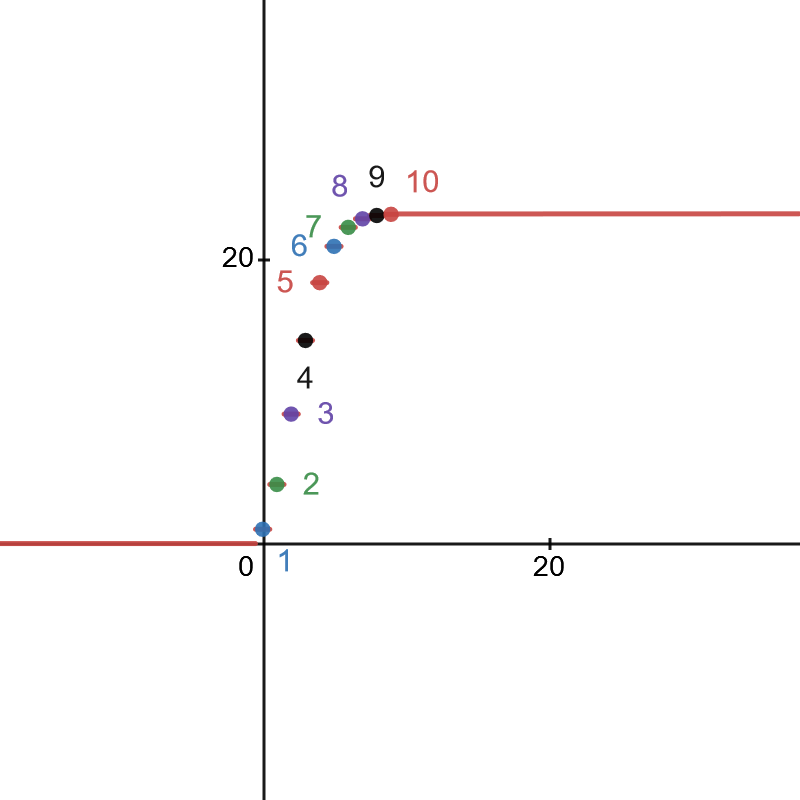
\includegraphics[width=\textwidth]{exponentialpowerseries.png}
	\caption{$e^z$ Power Series for $z = 3.14$}
	\end{subfigure}
\end{figure}

\end{flushleft}
\end{document}